\begin{figure}[H]
\centering
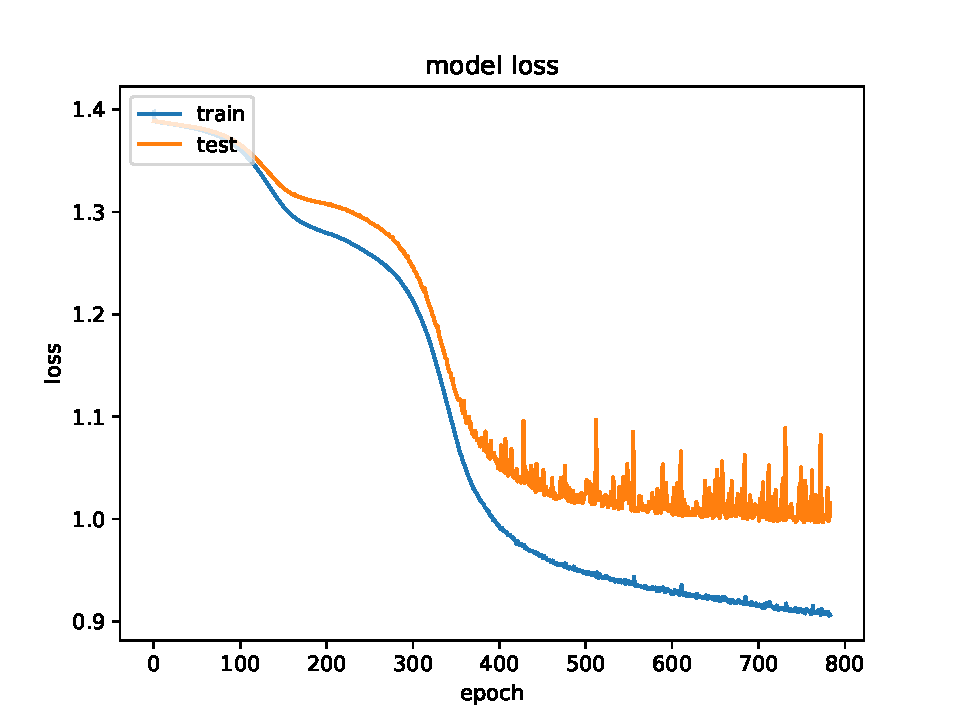
\includegraphics[width=0.45\textwidth]{\FCNCFigures/loss/lephad2jeven.pdf}
\put(-130, 115){\textbf{STH $\tlhad$ even}}
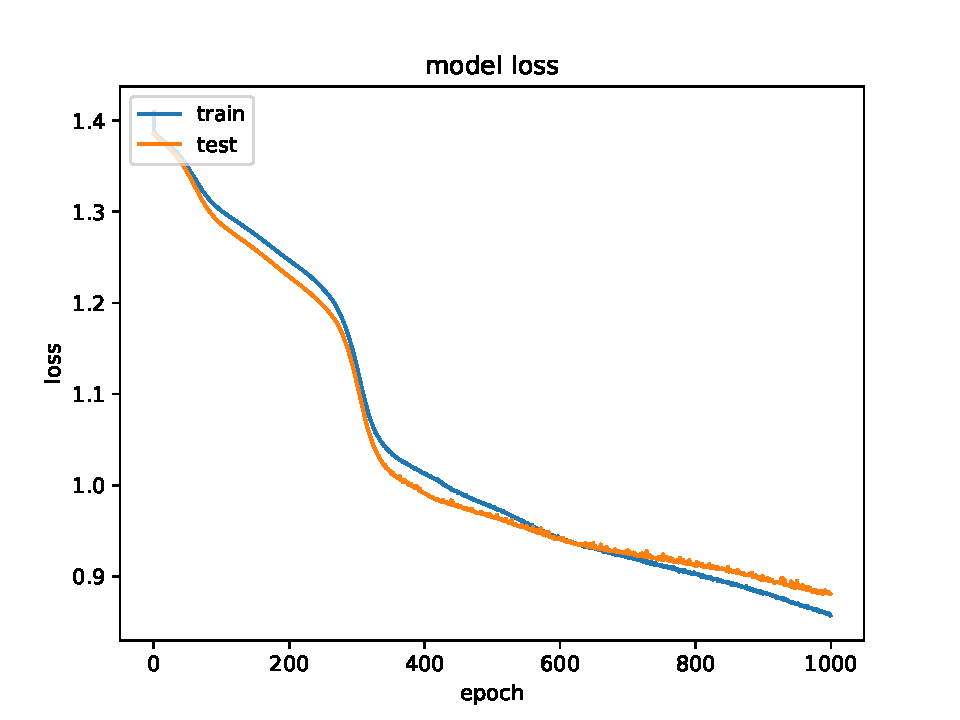
\includegraphics[width=0.45\textwidth]{\FCNCFigures/loss/lephad2jodd.pdf}
\put(-130, 115){\textbf{STH $\tlhad$ odd}}\\
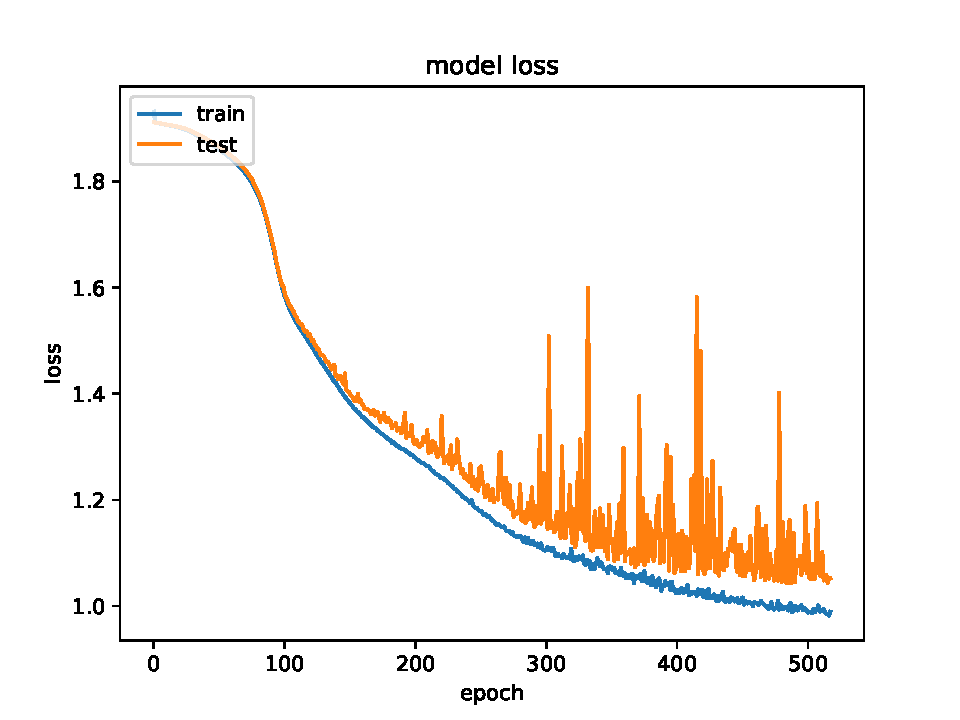
\includegraphics[width=0.45\textwidth]{\FCNCFigures/loss/lephad3jeven.pdf}
\put(-130, 115){\textbf{TTH $\tlhad$} 3j even}
\includegraphics[width=0.45\textwidth]{\FCNCFigures/loss/lephad3jodd.pdf}
\put(-130, 115){\textbf{TTH $\tlhad$} 3j odd}\\
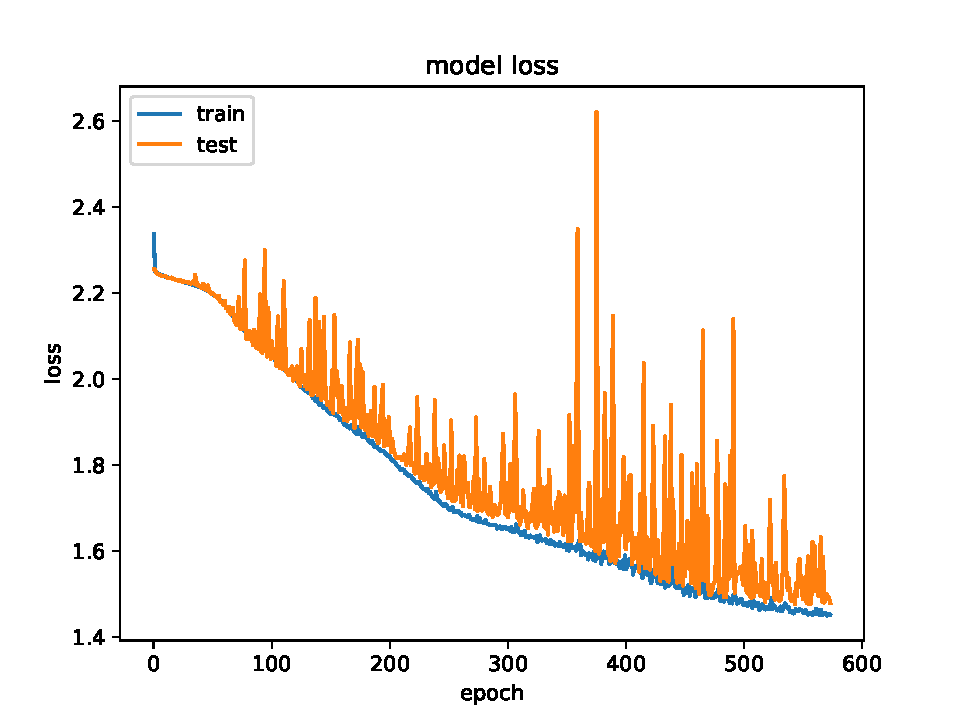
\includegraphics[width=0.45\textwidth]{\FCNCFigures/loss/lephad4jeven.pdf}
\put(-130, 115){\textbf{TTH $\tlhad$} 4j even}
\includegraphics[width=0.45\textwidth]{\FCNCFigures/loss/lephad4jodd.pdf}
\put(-130, 115){\textbf{TTH $\tlhad$} 4j odd}
\caption{各信号区神经网络训练的损失函数。}
\label{fig:loss_1}
\end{figure}

\begin{figure}[H]
\centering
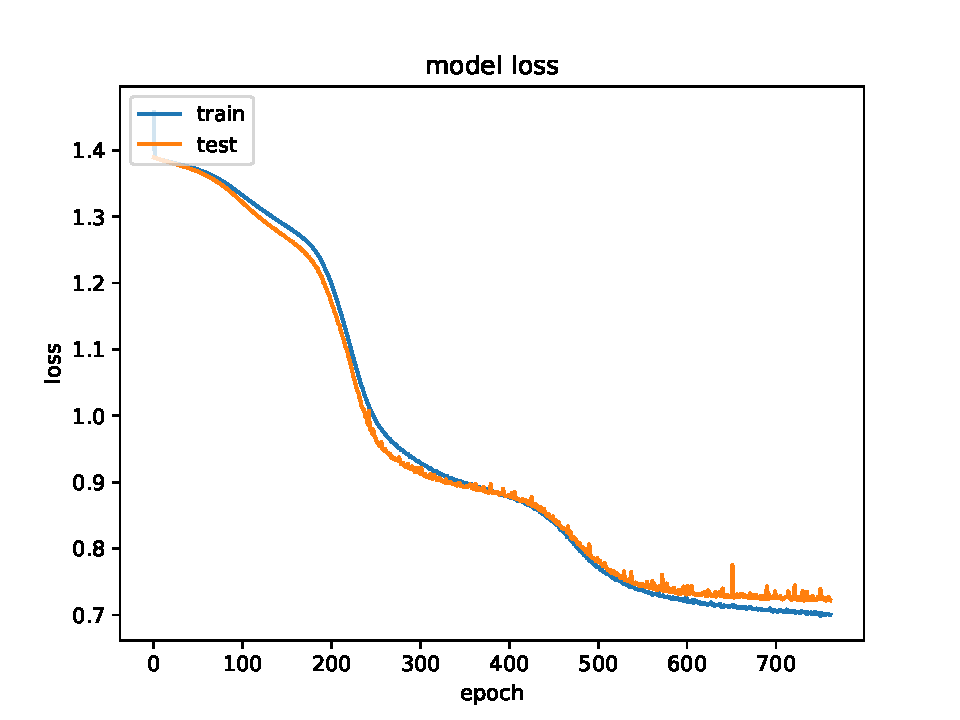
\includegraphics[width=0.45\textwidth]{\FCNCFigures/loss/lep2tau2jeven.pdf}
\put(-130, 115){\textbf{$l\thadhad$} 2j even}
\includegraphics[width=0.45\textwidth]{\FCNCFigures/loss/lep2tau2jodd.pdf}
\put(-130, 115){\textbf{$l\thadhad$} 2j odd}\\
\includegraphics[width=0.45\textwidth]{\FCNCFigures/loss/lep2tau3jeven.pdf}
\put(-130, 115){\textbf{$l\thadhad$} 3j even}
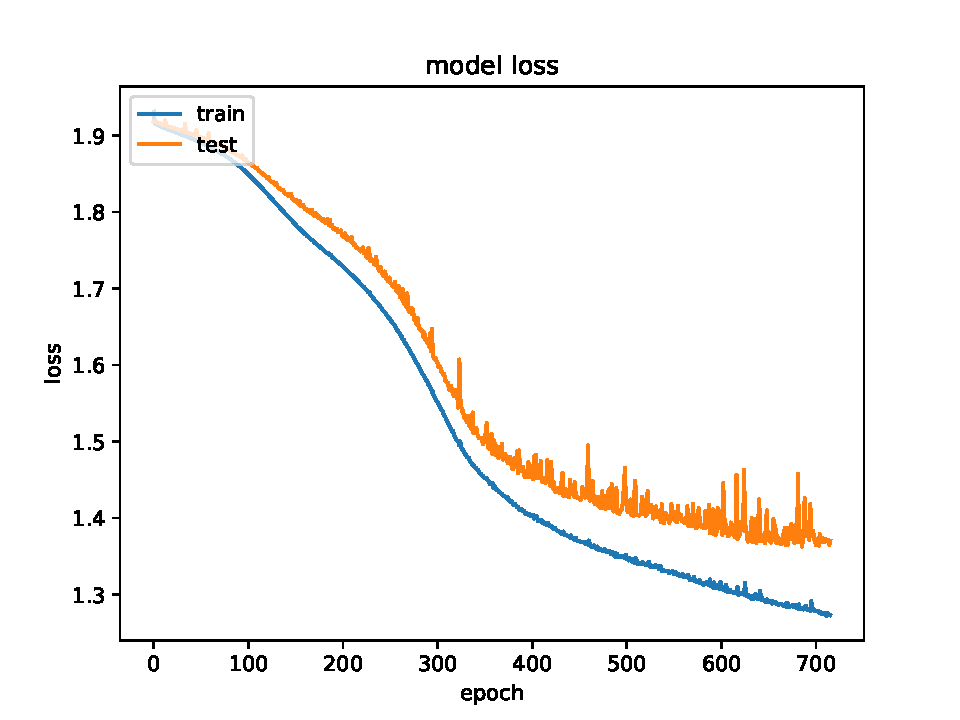
\includegraphics[width=0.45\textwidth]{\FCNCFigures/loss/lep2tau3jodd.pdf}
\put(-130, 115){\textbf{$l\thadhad$} 3j odd}
\caption{各信号区神经网络训练的损失函数。}
\label{fig:loss_2}
\end{figure}

